Исследуем диаметры интерференционных
колец, предполагая для простоты, что углы $\theta$ достаточно малы. Рассмотрим два
\begin{figure}[h!]
  \center{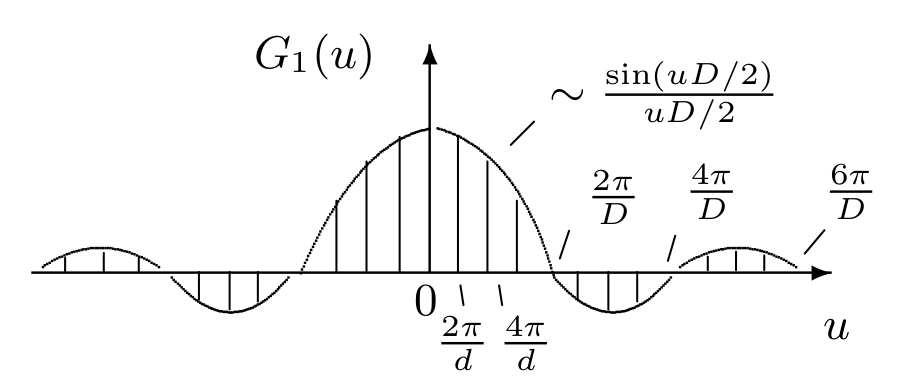
\includegraphics[width=\linewidth]{2.png}}
  \caption{Распределение интенсивности в проходящем свете в зависимости от порядка интерференции $\frac{\Delta}{\lambda}$}
  \label{img::2}
\end{figure}
\noindent интерференционных кольца, для которых порядки 
интерференции $\frac{\Delta}{\lambda}$ равны $m_i$ и $m_j$. Из формул \eqref{eq::1} и 
\eqref{eq::4} следует, что светлое кольцо порядка $m$ образуется при
\begin{equation}\label{eq::5}
  \Delta = 2L\cos{\theta} = m\lambda \: \: 
  \text{($m$ -- целое).}
\end{equation}
\noindent Отметим, что порядок интерференции возрастает при переходе к
кольцам меньшего диаметра, т.~е. при уменьшении угла $\theta$.

При малых $\theta$ имеем
\begin{equation}\label{eq::6}
  2L\left(1 - \frac{\theta_i^2}{2}\right) = m_i\lambda; \: \:
  2L\left(1 - \frac{\theta_j^2}{2}\right) = m_j\lambda.
\end{equation}
\noindent Вычитая второе уравнение из первого и принимая во внимание, 
что при переходе к соседнему кольцу порядок интерференции 
меняется на единицу, получим
$$
L\left(\theta_j^2 - \theta_i^2\right) = 
\left(m_i - m_j\right)\lambda = \left(j - i\right)\lambda.
$$
\noindent В приведённой формуле номера колец $i$ и $j$ отсчитываются от центра.

Диаметр $D$ кольца в фокальной плоскости линзы $Л$ связан с её 
фокусным расстоянием $f$ соотношением
\begin{equation}\label{eq::7}
  D = 2f\theta.
\end{equation}
\noindent Следовательно,
\begin{equation}\label{eq::8}
  \lambda = \frac{L}{4f^2}\frac{D_j^2 - D_i^2}{j - i}.
\end{equation}
\noindent Эта формула используется при измерении длины волны 
света с помощью интерферометра Фабри–Перо или для определения 
постоянной интерферометра $L$ по известному значению $\lambda$.

Пусть теперь в интерферометре Фабри–Перо наблюдается система
колец для двух близких спектральных линий $\lambda$ и $\lambda+d\lambda$. 
Дифференцируя \eqref{eq::5}, при малых $\theta$ найдём
$$
-2L\theta d \theta = md\lambda,
$$
\noindent откуда следует:
\begin{equation}\label{eq::9}
  d\lambda = - \frac{2L\theta}{m}d\theta \simeq -\lambda\theta d\theta 
  = - \frac{\lambda\overline{D}}{4f^2}dD,
\end{equation}
\noindent где $\overline{D}$ -- средний диаметр колец, a $dD$
-- разность диаметров колец, образующихся для спектральных линий 
с длинами волн $\lambda$, и $\lambda + d\lambda$ при одинаковом 
порядке интерференции. С помощью формулы \eqref{eq::9} можно
определять $d\lambda$, не зная постоянной интерферометра $L$.
Выбирая прибор для исследования спектра, обычно сравнивают три
характеристики: \textit{дисперсию}, \textit{дисперсионную область} и
\textit{разрешающую способность}.